\documentclass{beamer}\usepackage[]{graphicx}\usepackage[]{color}
%% maxwidth is the original width if it is less than linewidth
%% otherwise use linewidth (to make sure the graphics do not exceed the margin)
\makeatletter
\def\maxwidth{ %
  \ifdim\Gin@nat@width>\linewidth
    \linewidth
  \else
    \Gin@nat@width
  \fi
}
\makeatother

\definecolor{fgcolor}{rgb}{1, 0.894, 0.769}
\newcommand{\hlnum}[1]{\textcolor[rgb]{0.824,0.412,0.118}{#1}}%
\newcommand{\hlstr}[1]{\textcolor[rgb]{1,0.894,0.71}{#1}}%
\newcommand{\hlcom}[1]{\textcolor[rgb]{0.824,0.706,0.549}{#1}}%
\newcommand{\hlopt}[1]{\textcolor[rgb]{1,0.894,0.769}{#1}}%
\newcommand{\hlstd}[1]{\textcolor[rgb]{1,0.894,0.769}{#1}}%
\newcommand{\hlkwa}[1]{\textcolor[rgb]{0.941,0.902,0.549}{#1}}%
\newcommand{\hlkwb}[1]{\textcolor[rgb]{0.804,0.776,0.451}{#1}}%
\newcommand{\hlkwc}[1]{\textcolor[rgb]{0.78,0.941,0.545}{#1}}%
\newcommand{\hlkwd}[1]{\textcolor[rgb]{1,0.78,0.769}{#1}}%
\let\hlipl\hlkwb

\usepackage{framed}
\makeatletter
\newenvironment{kframe}{%
 \def\at@end@of@kframe{}%
 \ifinner\ifhmode%
  \def\at@end@of@kframe{\end{minipage}}%
  \begin{minipage}{\columnwidth}%
 \fi\fi%
 \def\FrameCommand##1{\hskip\@totalleftmargin \hskip-\fboxsep
 \colorbox{shadecolor}{##1}\hskip-\fboxsep
     % There is no \\@totalrightmargin, so:
     \hskip-\linewidth \hskip-\@totalleftmargin \hskip\columnwidth}%
 \MakeFramed {\advance\hsize-\width
   \@totalleftmargin\z@ \linewidth\hsize
   \@setminipage}}%
 {\par\unskip\endMakeFramed%
 \at@end@of@kframe}
\makeatother

\definecolor{shadecolor}{rgb}{.97, .97, .97}
\definecolor{messagecolor}{rgb}{0, 0, 0}
\definecolor{warningcolor}{rgb}{1, 0, 1}
\definecolor{errorcolor}{rgb}{1, 0, 0}
\newenvironment{knitrout}{}{} % an empty environment to be redefined in TeX

\usepackage{alltt}
\usepackage{../371g-slides}
\title{Multiple Regression 2}
\subtitle{Lecture 8}
\author{STA 371G}
\IfFileExists{upquote.sty}{\usepackage{upquote}}{}
\begin{document}
  
  
  

  \frame{\maketitle}

  % Show outline at beginning of each section
  \AtBeginSection[]{ 
    \begin{frame}<beamer>
      \tableofcontents[currentsection]
    \end{frame}
  }

  %%%%%%% Slides start here %%%%%%%

  \begin{darkframes}
  
  
    \begin{frame}[fragile]{Predicting House prices in the Greater Boston Area}
      \fontsize{9}{9}\selectfont
      
      Median house price for each census tract, along with other data. \pause
      
      The final model:
      
\begin{knitrout}
\definecolor{shadecolor}{rgb}{0.137, 0.137, 0.137}\begin{kframe}
\begin{alltt}
\hlstd{> }\hlstd{model} \hlkwb{<-} \hlkwd{lm}\hlstd{(MEDV} \hlopt{~} \hlstd{CRIME}\hlopt{+}\hlstd{ZONE}\hlopt{+}\hlstd{NOX}\hlopt{+}\hlstd{ROOM}\hlopt{+}\hlstd{DIST}
\hlstd{+ }                  \hlopt{+}\hlstd{RADIAL}\hlopt{+}\hlstd{TAX}\hlopt{+}\hlstd{PTRATIO}\hlopt{+}\hlstd{LSTAT,} \hlkwc{data}\hlstd{=boston)}
\end{alltt}
\end{kframe}
\end{knitrout}
      \begin{columns}[onlytextwidth]
        \column{.5\textwidth}
          \begin{itemize}
            \item MEDV: Median Price (response)
            \item CRIME: Per capita crime rate
            \item ZONE: Proportion of large lots
            \item NOX: Nitrogen Oxide concentration
            \item DIST: Distance to employment centers
          \end{itemize}
        \column{.5\textwidth}
          \begin{itemize}
            \item ROOM: Average \# of rooms
            \item RADIAL: Accessibility to highways
            \item TAX: Tax rate (per \$10K)
            \item PTRATIO: Pupil-to-teacher ratio
            \item LSTAT: Proportion of ``lower status''
            %  proportion of adults without some high school education or that are classified as laborers
          \end{itemize}
      \end{columns}
    \end{frame}
    
   
   
    \begin{frame}[fragile]{Overall Null Hypothesis}
      \fontsize{9}{9}\selectfont
    
      Is our model useful? Check the R-squared:
\begin{knitrout}
\definecolor{shadecolor}{rgb}{0.137, 0.137, 0.137}\begin{kframe}
\begin{alltt}
\hlstd{> }\hlkwd{summary}\hlstd{(model)}\hlopt{$}\hlstd{r.squared}
\end{alltt}
\begin{verbatim}
[1] 0.7282911
\end{verbatim}
\end{kframe}
\end{knitrout}
      \quad \pause
      
      Can we be confident that our model will generalize to the \alert{population}?  \pause
      
      \bigskip
      
      $H_0: \beta_1=\beta_2=\beta_3=\beta_4=\beta_5=\beta_6=\beta_7=\beta_8=\beta_9=0$ (Data explains nothing!) \pause
      
      $H_1: \beta_i \neq 0$ for some $i$ (At least one predictor is useful) \pause
      
      \bigskip
      
      or 
      
      \bigskip
      
      $H_0: R^2=0$
      
      $H_1: R^2>0$
    \end{frame}
   
   
   
   \begin{frame}[fragile]{Overall Null Hypothesis}
      \fontsize{9}{9}\selectfont
      Check the P-value for the  F-statistic in the summary
      \begin{center}
        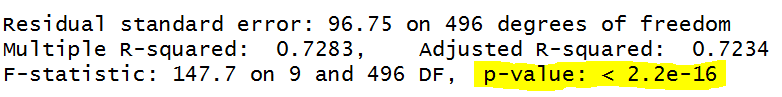
\includegraphics[width=4in]{r_sq_pval} \\
      \end{center}
      So we can reject the overall null hypothesis! \pause
      
      R-squared was already too big to suspect that it is zero and we already knew some predictors are statistically significant.
      
    \end{frame}  
   
   
    
    \begin{frame}[fragile]{How good are our predictions?}
      \fontsize{9}{9}\selectfont
      Let's plot the residuals, i.e., discrepancies between the predictions and the data. \pause
      
\begin{knitrout}
\definecolor{shadecolor}{rgb}{0.137, 0.137, 0.137}\begin{kframe}
\begin{alltt}
\hlstd{> }\hlkwd{hist}\hlstd{(model}\hlopt{$}\hlstd{residuals,} \hlkwc{col}\hlstd{=}\hlstr{'green'}\hlstd{,}
\hlstd{+ }  \hlkwc{main}\hlstd{=}\hlstr{''}\hlstd{,} \hlkwc{xlab}\hlstd{=}\hlstr{'Residuals (in $1K)'}\hlstd{,} \hlkwc{ylab}\hlstd{=}\hlstr{'Frequency'}\hlstd{)}
\end{alltt}
\end{kframe}
\input{C:/temp/figures/unnamed-chunk-5-1.tikz}

\end{knitrout}
      
      
    \end{frame}  
    
    
    \begin{frame}[fragile]{How good are our predictions?}
      \fontsize{9}{9}\selectfont
      It looks like a normal distribution. Let's look at the mean of the residuals: \pause
      
\begin{knitrout}
\definecolor{shadecolor}{rgb}{0.137, 0.137, 0.137}\begin{kframe}
\begin{alltt}
\hlstd{> }\hlkwd{mean}\hlstd{(model}\hlopt{$}\hlstd{residuals)}
\end{alltt}
\begin{verbatim}
[1] -2.028049e-15
\end{verbatim}
\end{kframe}
\end{knitrout}
      Virtually zero. \pause

      \bigskip
      (It will be always zero since regression minimizes the sum of squared residuals.) \pause
      
      \bigskip
      
      What about the standard deviation? \pause
\begin{knitrout}
\definecolor{shadecolor}{rgb}{0.137, 0.137, 0.137}\begin{kframe}
\begin{alltt}
\hlstd{> }\hlkwd{sd}\hlstd{(model}\hlopt{$}\hlstd{residuals)}
\end{alltt}
\begin{verbatim}
[1] 95.88111
\end{verbatim}
\end{kframe}
\end{knitrout}
      \pause
      By the 2 standard deviation rule, we could estimate that 95\% of the time residuals are in [-\$192K, \$192K] range.
    \end{frame}  
   
    
    \begin{frame}[fragile]{How good are our predictions?}
      \fontsize{9}{9}\selectfont
      
      Can we obtain a \alert{similar} measure directly from the summary of the regression?
      
      \note{Emphasize that standard error and what we get with sd() is similar, but not exactly the same. 
           sd() estimates the population std dev, standard error is obtained by dividing SS by the num. deg. of freedom. } \pause
           
      It is the Residual standard error!
\begin{knitrout}
\definecolor{shadecolor}{rgb}{0.137, 0.137, 0.137}\begin{kframe}
\begin{alltt}
\hlstd{> }\hlkwd{summary}\hlstd{(model)}\hlopt{$}\hlstd{sigma}
\end{alltt}
\begin{verbatim}
[1] 96.74708
\end{verbatim}
\end{kframe}
\end{knitrout}
      \quad \pause
      \begin{center}
        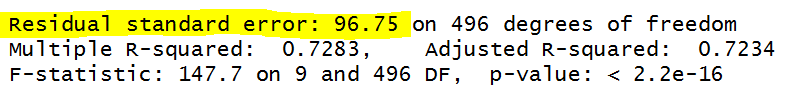
\includegraphics[width=4in]{std_err} \\
      \end{center}
      
    \end{frame}
    
    
    
    \begin{frame}{Again: regression assumptions}
      Remember the big four:
      \begin{enumerate}
        \item \alert{The residuals are independent.}
        \item $Y$ is a linear function of $X$s (except for the errors).
        \item The residuals are normally distributed.
        \item The variance of $Y$ is the same for any value of $X$s (``homoscedasticity'').
    
      \end{enumerate}
    \end{frame}
    
    
    \begin{frame}[fragile]{Assumption 1: Independence}
      Independence: No correlation between residuals. \pause
    
      Difficult to verify this from plots.
      
    \end{frame}
    

    
    
    
    \begin{frame}{Again: regression assumptions}
      Remember the big four:
      \begin{enumerate}
        \item The residuals are independent.
        \item \alert{$Y$ is a linear function of $X$s (except for the errors).}
        \item The residuals are normally distributed.
        \item The variance of $Y$ is the same for any value of $X$s (``homoscedasticity'').
      \end{enumerate}
    \end{frame}
    
    
    
    \begin{frame}[fragile]{Assumption 2: Linearity}
    
      Plot the residuals vs the predicted Y-values and ensure there is no trend:
\begin{knitrout}
\definecolor{shadecolor}{rgb}{0.137, 0.137, 0.137}\begin{kframe}
\begin{alltt}
\hlstd{> }\hlkwd{plot}\hlstd{(}\hlkwd{predict.lm}\hlstd{(model),} \hlkwd{resid}\hlstd{(model),}
\hlstd{+ }  \hlkwc{xlab}\hlstd{=}\hlstr{'Predicted values'}\hlstd{,} \hlkwc{ylab}\hlstd{=}\hlstr{'Residuals'}\hlstd{)}
\end{alltt}
\end{kframe}
\input{C:/temp/figures/unnamed-chunk-9-1.tikz}

\end{knitrout}
    \end{frame}   
    
    
    \begin{frame}{Again: regression assumptions}
      Remember the big four:
      \begin{enumerate}
        \item The residuals are independent.
        \item $Y$ is a linear function of $X$s (except for the errors).
        \item \alert{The residuals are normally distributed.}
        \item The variance of $Y$ is the same for any value of $X$s (``homoscedasticity'').
      \end{enumerate}
    \end{frame}
    
    
    
    \begin{frame}[fragile]{Assumption 3: Normally distributed residuals}
      Ensure that the Q-Q plot shows a (roughly) straight line:
\begin{knitrout}
\definecolor{shadecolor}{rgb}{0.137, 0.137, 0.137}\begin{kframe}
\begin{alltt}
\hlstd{> }\hlkwd{qqnorm}\hlstd{(}\hlkwd{resid}\hlstd{(model),} \hlkwc{main}\hlstd{=}\hlstr{''}\hlstd{)}
\end{alltt}
\end{kframe}
\input{C:/temp/figures/unnamed-chunk-10-1.tikz}

\end{knitrout}
    \end{frame}
    
    
    \begin{frame}{Again: regression assumptions}
      Remember the big four:
      \begin{enumerate}
        \item The residuals are independent.
        \item $Y$ is a linear function of $X$s (except for the errors).
        \item The residuals are normally distributed.
        \item \alert{The variance of $Y$ is the same for any value of $X$s (``homoscedasticity'').}
      \end{enumerate}
    \end{frame}
    
    
    \begin{frame}[fragile]{Assumption 4: The variance of $Y$ is the same across}
      Look for a (roughly) constant vertical ``thickness'':  
\begin{knitrout}
\definecolor{shadecolor}{rgb}{0.137, 0.137, 0.137}\begin{kframe}
\begin{alltt}
\hlstd{> }\hlkwd{plot}\hlstd{(}\hlkwd{predict.lm}\hlstd{(model),} \hlkwd{resid}\hlstd{(model),}
\hlstd{+ }  \hlkwc{xlab}\hlstd{=}\hlstr{'Predicted values'}\hlstd{,} \hlkwc{ylab}\hlstd{=}\hlstr{'Residuals'}\hlstd{)}
\end{alltt}
\end{kframe}
\input{C:/temp/figures/unnamed-chunk-11-1.tikz}

\end{knitrout}
    \end{frame}
    
    
    
    
    \begin{frame}[fragile]{We have a model. Then what?}
    
      Let's make some predictions.
    \end{frame}
    
    
    \begin{frame}[fragile]{Model Coefficients}
      Regression model estimates the coefficients of the predictors.
\begin{knitrout}
\definecolor{shadecolor}{rgb}{0.137, 0.137, 0.137}\begin{kframe}
\begin{alltt}
\hlstd{> }\hlkwd{round}\hlstd{(}\hlkwd{summary}\hlstd{(model)}\hlopt{$}\hlstd{coefficients,}\hlnum{2}\hlstd{)}
\end{alltt}
\begin{verbatim}
            Estimate Std. Error t value Pr(>|t|)
(Intercept)   840.07      99.00    8.49        0
CRIME          -2.57       0.66   -3.87        0
ZONE            0.92       0.28    3.34        0
NOX          -346.93      71.81   -4.83        0
ROOM           74.24       8.26    8.99        0
DIST          -31.05       3.78   -8.20        0
RADIAL          6.00       1.29    4.66        0
TAX            -0.27       0.07   -3.87        0
PTRATIO       -19.28       2.63   -7.34        0
LSTAT         -11.07       0.96  -11.56        0
\end{verbatim}
\end{kframe}
\end{knitrout}
      
    \end{frame}
    
    
    
    
      \begin{frame}[fragile]{Model Coefficients}
      Let's estimate the median house price in a district, where:
      
      \begin{table}[!b]
        {\carlitoTLF % Use monospaced lining figures
        \begin{tabularx}{\textwidth}{XXrrr}
           
           $j$ & Predictor  & $\beta_j$   &  $X_j$  & $\beta_j X_j$ \\ 
          \toprule
            0 & Intercept	&	840.07	&	1	&	840.07  \\
            1 & CRIME	&	-2.57	&	0.03	&	-0.0771  \\
            2 & ZONE	&	0.92	&	10	&	9.2  \\
            3 & NOX	&	-346.93	&	0.5	&	-173.465  \\
            4 & ROOM	&	74.24	&	4	&	296.96  \\
            5 & DIST	&	-31.05	&	5	&	-155.25  \\
            6 & RADIAL	&	6	&	1	&	6  \\
            7 & TAX	&	-0.27	&	300	&	-81  \\
            8 & PTRATIO	&	-19.28	&	15	&	-385.6  \\
            9 & LSTAT	&	-11.07	&	10	&	-110.7  \\
          \bottomrule
             Price &  Estimate 	& (\$1000)		&		&	342.538   \\
        
        
        \end{tabularx}}
        
      \end{table} 
      
    \end{frame}



    \begin{frame}[fragile]{Model Coefficients}
      Let R do it for us!
      
\begin{knitrout}
\definecolor{shadecolor}{rgb}{0.137, 0.137, 0.137}\begin{kframe}
\begin{alltt}
\hlstd{> }\hlkwd{predict.lm}\hlstd{(model,} \hlkwd{list}\hlstd{(}\hlkwc{CRIME}\hlstd{=}\hlnum{0.03}\hlstd{,} \hlkwc{ZONE}\hlstd{=}\hlnum{10}\hlstd{,}
\hlstd{+ }                       \hlkwc{NOX}\hlstd{=}\hlnum{0.5}\hlstd{,} \hlkwc{ROOM}\hlstd{=}\hlnum{4}\hlstd{,}
\hlstd{+ }                       \hlkwc{DIST}\hlstd{=}\hlnum{5}\hlstd{,}  \hlkwc{RADIAL}\hlstd{=}\hlnum{1}\hlstd{,}
\hlstd{+ }                       \hlkwc{TAX}\hlstd{=}\hlnum{300}\hlstd{,} \hlkwc{PTRATIO}\hlstd{=}\hlnum{15}\hlstd{,}
\hlstd{+ }                       \hlkwc{LSTAT}\hlstd{=}\hlnum{10}\hlstd{))}
\end{alltt}
\begin{verbatim}
       1 
343.9552 
\end{verbatim}
\end{kframe}
\end{knitrout}
      \pause
      Cool! That was easy!
      \note{The discrepancy is due to rounding in the previous slide.}
      
    \end{frame}
    
    
    \begin{frame}[fragile]{Model Coefficients}
      Assume that there are 420 students and 28 teachers in the disctrict (that is why PTRATIO is 15). \pause
      
      \bigskip
      
      The school board is considering to hire 2 more teachers. How would this affect the house prices in the district? \pause
      
      \bigskip
      
      The new PTRATIO will be $420/30=14$. \pause
      
\begin{knitrout}
\definecolor{shadecolor}{rgb}{0.137, 0.137, 0.137}\begin{kframe}
\begin{alltt}
\hlstd{> }\hlkwd{predict.lm}\hlstd{(model,} \hlkwd{list}\hlstd{(}\hlkwc{CRIME}\hlstd{=}\hlnum{0.03}\hlstd{,} \hlkwc{ZONE}\hlstd{=}\hlnum{10}\hlstd{,}
\hlstd{+ }                       \hlkwc{NOX}\hlstd{=}\hlnum{0.5}\hlstd{,} \hlkwc{ROOM}\hlstd{=}\hlnum{4}\hlstd{,}
\hlstd{+ }                       \hlkwc{DIST}\hlstd{=}\hlnum{5}\hlstd{,}  \hlkwc{RADIAL}\hlstd{=}\hlnum{1}\hlstd{,}
\hlstd{+ }                       \hlkwc{TAX}\hlstd{=}\hlnum{300}\hlstd{,} \hlkwc{PTRATIO}\hlstd{=}\hlnum{14}\hlstd{,}
\hlstd{+ }                       \hlkwc{LSTAT}\hlstd{=}\hlnum{10}\hlstd{))}
\end{alltt}
\begin{verbatim}
       1 
363.2349 
\end{verbatim}
\end{kframe}
\end{knitrout}
    \end{frame}
    
    
    
    \begin{frame}[fragile]{Model Coefficients}
      Nothing is free. To be able to compansate the new hires, the ISD decides to add \$50 more on your tax bill for every \$10K of your house price. \pause
      
      \bigskip
      So, the tax rate increases to 350 per \$10K. How would this affect the median house price?
      
      \lc
    
    \end{frame}
    
    
    
    \begin{frame}[fragile]{Confidence intervals}
      We all know our predictions are wrong. 
      
      Can we come up with some confidence intervals on our predictions? \pause
      \bigskip
      
      Remember the two kinds of intervals:
      \bigskip

      \begin{tabular}{lp{1in}p{2in}}
        \textbf{Confidence} & Predicting the mean value of $Y$ for a particular  set of $X$ values. & Among all the districts whose predictors are as above, what is the mean value of median house price?  \\
        \textbf{Prediction} & Predicting $Y$ for a single new case. & If Springfield has the predictors above, what is the median house price in Springfield?\\
      \end{tabular}
    
    
    \end{frame}
        
      
    
    \begin{frame}[fragile]{Confidence intervals}
    
\begin{knitrout}
\definecolor{shadecolor}{rgb}{0.137, 0.137, 0.137}\begin{kframe}
\begin{alltt}
\hlstd{> }\hlkwd{predict.lm}\hlstd{(model,} \hlkwd{list}\hlstd{(}\hlkwc{CRIME}\hlstd{=}\hlnum{0.03}\hlstd{,} \hlkwc{ZONE}\hlstd{=}\hlnum{10}\hlstd{,}
\hlstd{+ }                       \hlkwc{NOX}\hlstd{=}\hlnum{0.5}\hlstd{,} \hlkwc{ROOM}\hlstd{=}\hlnum{4}\hlstd{,}
\hlstd{+ }                       \hlkwc{DIST}\hlstd{=}\hlnum{5}\hlstd{,}  \hlkwc{RADIAL}\hlstd{=}\hlnum{1}\hlstd{,}
\hlstd{+ }                       \hlkwc{TAX}\hlstd{=}\hlnum{350}\hlstd{,} \hlkwc{PTRATIO}\hlstd{=}\hlnum{14}\hlstd{,}
\hlstd{+ }                       \hlkwc{LSTAT}\hlstd{=}\hlnum{10}\hlstd{),}
\hlstd{+ }                       \hlkwc{interval} \hlstd{=} \hlstr{'confidence'}\hlstd{)}
\end{alltt}
\begin{verbatim}
       fit      lwr      upr
1 349.9684 301.9485 397.9883
\end{verbatim}
\end{kframe}
\end{knitrout}
     \lc
     \end{frame}
     
     
     
     \begin{frame}[fragile]%{Confidence intervals}
        We can also put a confidence intervals on a coefficient to estimate the range of its effect.
        
\begin{knitrout}
\definecolor{shadecolor}{rgb}{0.137, 0.137, 0.137}\begin{kframe}
\begin{alltt}
\hlstd{> }\hlkwd{confint}\hlstd{(model)}
\end{alltt}
\begin{verbatim}
                   2.5 %       97.5 %
(Intercept)  645.5520530 1034.5782470
CRIME         -3.8703245   -1.2618439
ZONE           0.3792933    1.4647029
NOX         -488.0175640 -205.8337804
ROOM          58.0099148   90.4751248
DIST         -38.4860994  -23.6129585
RADIAL         3.4693548    8.5311305
TAX           -0.4000457   -0.1306157
PTRATIO      -24.4415728  -14.1179304
LSTAT        -12.9529546   -9.1905075
\end{verbatim}
\end{kframe}
\end{knitrout}
     
     \end{frame}
     
     \begin{frame}[fragile]{Confidence intervals}
        Reducing the PTRATIO by one could increase the median house price from \$14K to \$24K!
        
        \lc
     \end{frame}
        
        
 
  \end{darkframes}

\end{document}
